%%%      1         2         3         4         5         6         7        8
%%% 567890123456789012345678901234567890123456789012345687901234567890123456790
%%%
%%% Introduction.
%%%

\svnInfo $Id$

\newcommand\schema[1]{\ensuremath{\mathcal{#1}}}
\newcommand\relation[1]{\ensuremath{\textnormal{\bf\textsf{#1}}}}

\makeatletter
\newcommand\skyline{\mathop{\operator@font skyline}\nolimits}
\newcommand\skyband{\mathop{\operator@font skyband}\nolimits}
\makeatother

\newcommand\imp{\Rightarrow}
\newcommand\bigland{\bigwedge}
\newcommand\biglor{\bigvee}
\newcommand\union{\cup}
\newcommand\bigunion{\bigcup}
\newcommand\intersection{\cap}
\newcommand\difference{\backslash}
\newcommand\dominates{\ensuremath{\succ}\xspace}
\newcommand\weakdominates{\ensuremath{\succeq}\xspace}

\newcommand\inlinesql[1]{{\tt #1}}
\newcommand\srcref[1]{{\tt #1}}
\newcommand\postgresdocu[2]{\href{http://www.postgresql.org/docs/8.3/static/#1}{#2}\footnote{\url{http://www.postgresql.org/docs/8.3/static/#1}}}
\newcommand\ttbackslash{{\char92}}

\newtheorem{definition}{Definition}
\newtheorem{lemma}{Lemma}
\newtheorem{theorem}{Theorem}

\newcommand\nt[1]{\textit{#1}}

\makeatletter
\newenvironment{interactive}
{%
\newcommand\shprompt[1]{\$\ {\textbf{##1}}}
\newcommand\sqlprompt[1]{db=\# {\textbf{##1}}}
\newcommand\sqlpromptcont[1]{db-\# {\textbf{##1}}}
\newcommand\comment[1]{{\rmfamily\textit{##1}}}
\newcommand\rcomment[1]{\hfill\comment{##1}}
\begingroup\small\list{}{\listparindent 0\p@\itemindent\listparindent\leftmargin15\p@\rightmargin15\p@}\item[]\begin{alltt}}{\end{alltt}\endlist\endgroup}

\newdimen\onecolumnwidth
\global\onecolumnwidth\textwidth
\advance\onecolumnwidth -\columnsep
\divide\onecolumnwidth\tw@
\newsavebox\tempbox

\makeatother

\newcommand\subplotprofile[2][todo]{%
\subfloat[#1]{%
\includegraphics[width=\onecolumnwidth]{plots-profile/#2}}%
}%

\newcommand\subplotlabeledprofile[3]{%
\subfloat[#1]{%
\includegraphics[width=\onecolumnwidth]{plots-profile/#2}%
\label{#3}%
}}%



\section{TODO}
\begin{itemize}
\item \todo{casing of section headings?}{}
\item \todo{ask ali, which website for travelling by airplane uses skyline}{}
\item \todo{using hashing for diff groups}{}
\item \todo{EF+SFS=LESS (check this again)}{}
\item \todo{has the order in which the skyline dimensions are checked an effect?}{}
\item \todo{show how Preference SQL ABOUT can be emulated}{}
\item \todo{PostgreSQL as of 8.3 does not derive the stats for subselect like \inlinesql{explain analyze select * from (select * from i15d1e6s0 limit 1000) as a skyline of d1 min, d2 min with windowpolicy=ranked;}}{}
\end{itemize}
\clearpage


\chapter{Introduction}
\label{chap:Introduction}


\section{General Introduction}
\todo{}{take some parts from the research planning intro}

\begin{figure}[htbp]
% this is from: 
% http://www.istockphoto.com/file_closeup/where/scenics/cityscapes/
% 2358169_lightning_traffic_over_danube_bridge_and_vienna_skyline.php
% ?id=2358169
%
% Photographers Description:
%
% viennese skyline with cars driving on a street shot by night with a
% long time exposure. I added high contrast, therefore image gets very
% little grainy.
%
\centering
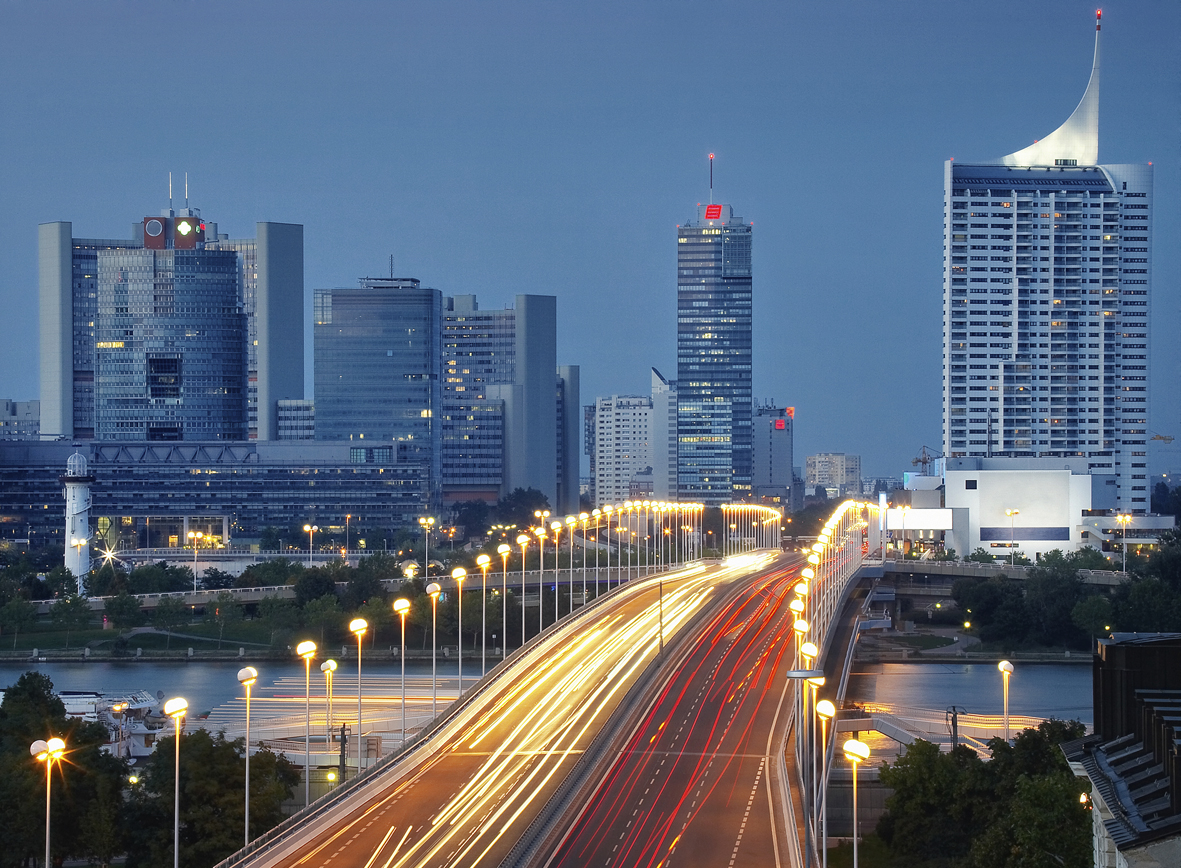
\includegraphics[scale=1.0]{photos/iStock_000002358169Large_100mm}%
\caption{Viennese skyline (nightshot with long exposure time, 
taken by Franz Pfl�gl / Vienna}%
\label{fig:vienneseskyline}%
\end{figure}

give the intuition.

\subsection{Typographical Conventions}
For interactive input and output we will show our typed input in a \texttt{\bfseries bold font}, the output \texttt{like this}, \textit{and comments like this}.


%         1         2         3         4         5         6         7         8
%12345678901234567890123456789012345678901234567890123456789012345678901234567890

\begin{interactive}
\shprompt{psql}\rcomment{start PostgreSQL interactive terminal}
\sqlprompt{SELECT * FROM a2d1e5s0 SKYLINE OF d1 MIN, d2 MIN;}\rcomment{issue a skyline query}
  id   |          d1           |          d2
-------+-----------------------+-----------------------
   417 |     0.660430708919594 |    0.0734207719527077
  1329 |    0.0486199019148477 |     0.663867116113964
...\rcomment{53 rows omitted}
 98953 |     0.136247931652335 |     0.607638615081091
(56 rows)

\sqlprompt{\ttbackslash{}q}\rcomment{quit psql}
\shprompt{}\rcomment{back at the shell prompt}
\end{interactive}

The example above also illustrates two other concepts: ``\texttt{\$}''
indicates a shell prompt and ``\texttt{db=\#}'' indicates the prompt for
PostgreSQL interactive terminal \texttt{psql}. Furthermore
``\texttt{db-\#}'' is displayed when \texttt{psql} is waiting for more
input. All of them are used throughtout the text.

\subsection{motivation}
motivation: green computing: less cpu time, less computers, less
energy --> safe the planet

stocks: risk vs. costs (--> streaming skyline see [Tao2006])

example of skyline

when travelling by airplane: time vs. costs

TODO: more dim: \#stops, total dist
travel by bus: \#of visited cities

it is shown on some website. which?

Credit To: Ali (room mate)

employee (salary, revenue, years in the company)

\subsection{consider only bnl and sfs}

from \citep{Chaudhuri2006}:

In this paper, our focus is on algorithms that can be
directly implemented in today's commercial database systems
without the addition of new access methods (which
would require addressing the associated challenges of maintenance
with updates, concurrency control, etc.). Specifically,
we consider the Block-nested-loop Algorithm [15],
and the Block-nested-loop with Presorting [5].

Special algorithms have been proposed for the case the whole relation fits into main memory \citep{Preparata1985}, nevertheless we do not take them into account as memory is always a short resource in a database scenario, either due to the number of concurrent users or limited total main memory, e.g. on a handheld device.

The skyline operator \citep{Borzsonyi2001} filters out the \emph{interesting} points from a potentially large set of data points. The skyline operator returns the pareto optimal\index{pareto optimal} elements of a set. This is also know as maximum vector problem\index{maximum vector problem}.

\section{Related Problems}
Convex hull, \emph{top-K} queries, and nearest-neighbor search (especially in the context of spacial skylines ``give me the next good restaurant'')

In particlar, the convex hull contains the subset of skyline points that may be optimal only for linear preference functions (as opposed to any monotone function).\todo{from \citep{Papadias2005}}{rephrase}





\clearpage 
\fixme{}{no clearpage}
\section{Basic definitions}
\todo{We are in the context of relational model\index{relational model} of data}{\citep{Chomicki2002, Chomicki2003a}?}. As we aim at an implementation of the skyline operator into a relational database management system (RDBMS)\index{RDBMS} we restrict to finite database\index{finite database} instances.

We assume two \todo{infinite}{hm? although in a real computer is everything finte} domains: $N$ (numbers) and $D$ (uninterpreted constants). The domain $D$ will be used for attributes which are not subject to skyline computation, i.e. for the travelling example we will not use the name of the airline as a skyline criterion, therefore $D$ will be used as domain for this attribute.
For attributes or expressions which are subject to skyline computation we use the domain $N$. No distinction is made between different numeric domains, since it is not necessary for this paper. For $N$ we require that equality ($=$), inequality ($\not=$), and the binary relations $<$ (strictly less than), $\le$ (less than or equal), $\ge$ (greater than or equal), and $>$ (strictly greater than) are defined with the usual properties.

\begin{definition}[Schema]
Given the domains $U_i, 1 \le i \le n$, such that $U_i$ is either equal to $D$ or $N$, we define the $n$-ary schema $\schema{R}$ as the cartesian product of the $U_i$'s, i.e. $\schema{R} = U_1 \times U_2 \times \ldots \times U_n$. The attributes of schema \schema{R} will be refered as $a_1, \ldots, a_n$.
\end{definition}

Preferences will be defined in terms of \emph{binary preference relations}\index{preference relation}.
\begin{definition}[Preference relation]
Let \schema{R} be a $n$-ary schema, a relation \dominates is a preference relation over \schema{R} if it is a subset of $\schema{R} \times \schema{R}$.
\end{definition}

To give an intuition, \dominates will be a binary relation between pairs of tuples from the same (database) relation, we say $r$ \emph{dominates} $s$ in \dominates iff $(r, s) \in \dominates$ (or in infix notation $r \dominates s$).

We require the relation \dominates to be a \emph{strict partial order}\index{strict partial order}, i.e. \dominates is irreflexive, asymmetric and transitive. These properties are formalized as usual:

\begin{itemize}
\item \emph{irreflexivity:} $\forall x: x \not\dominates x$
\item \emph{asymmetry:} $\forall x, y: x \dominates y \imp y \not\dominates x$
\item \emph{transitivity:} $\forall x, y, z: (x \dominates y \land y \dominates z) \imp x \dominates z$
\end{itemize}

Non-transitive\index{non-transitive} preferences can be compute with the \todo{Best}{special font for algo names?} algorithm (\citep{Torlone2002, Ciaccia2004}), we will not study this approach in this paper.

\begin{definition}
\todo{}{}Let \relation{R} be a relation of schema \schema{R}.
\end{definition}

\begin{definition}[Skyline]
The skyline of a relation \relation{R} with respect to the preference relation \dominates is the set of tuples $r \in \relation{R}$ which are not dominate by any other tuple $s \in \relation{R}$, formally $\skyline_\dominates(\relation{R}) := \{ r \in \relation{R} | \nexists s \in \relation{R} : s \dominates r \}$
\end{definition}

\begin{lemma}
\todo{}{this is more or less theorem 2 from \citep{Chomicki2002}}
Given the relation $\relation{R} \not= \emptyset$ and \dominates a strict parial order over \schema{R}, where \schema{R} is the schema for \relation{R}, the skyline is non empty, i.e. $\skyline_\dominates(\relation{R}) \not= \emptyset$ holds.
\end{lemma}


In a skyline query with the following skyline clause:
\todo{}{add space between dim and direction}
\[
\texttt{SKYLINE OF} a_1 \texttt{MIN}, \ldots, a_k \texttt{MIN}, a_{k+1} \texttt{MAX}, \ldots, a_l \texttt{MAX}, a_{l+1} \texttt{DIFF}, \ldots, a_m \texttt{DIFF}
\]
a tuple 
$r = (r_1, \ldots, r_k, r_{k+1}, \ldots, r_l, r_{l+1}, \ldots, r_m, r_{m+1}, \ldots, r_n)$
dominates a tuple
$s = (r_1, \ldots, r_k, r_{k+1}, \ldots, r_l, r_{l+1}, \ldots, r_m, r_{m+1}, \ldots, r_n)$
iff the following condition holds
\begin{eqnarray}\label{equ:skylinepf}
\left( \bigland_{1 \le i \le k} r_i \le s_i \right) \land
\left( \bigland_{k+1 \le i \le l} r_i \ge s_i \right) \land
\left( \bigland_{l+1 \le i \le m} r_i = s_i \right) \land \nonumber\\
\land
\left( \left( \biglor_{1 \le i \le k} r_i < s_i \right) \lor
       \left( \biglor_{k+1 \le i \le l} r_i > s_i \right) \right).
\end{eqnarray}

To state in an informal way, a tuple $r$ dominates a tuple $s$ if it is equal in all \inlinesql{DIFF} dimensions, at least as good in all \inlinesql{MIN}/\inlinesql{MAX} dimensions and better than in at least one of the \inlinesql{MIN}/\inlinesql{MAX} dimensions.

\todo{make \dominates equal to (\ref{equ:skylinepf}) and \weakdominates equal to just the $\le$ part, use $r \sim s := r \weakdominates s \land s \weakdominates r = \forall i \in \{1, \ldots, m\}: r_i = s_i$, i.e. equal on all skyline dimensions}{}


If $\forall i \in \{1, \ldots, m\}: r_i = s_i$ holds, $r$ and $s$ are \todo{\emph{incomparable}}{use an other term for this special case of incomparability}, if \inlinesql{DISTINCT} is specified it is left up to the implementation to include either $r$ or $s$ in the skyline, if \inlinesql{DISTINCT} is not specified $r$ and $s$ are included. 


In case condition (\ref{equ:skylinepf}) does not hold $r$ and $s$ are \emph{incomparable} and may both be part of the skyline if not dominated by any other tuple from \relation{R}.

Please note that the following subformula (\ref{equ:skylinepfdiff}) of formula (\ref{equ:skylinepf}) induces an equality relation on \relation{R}, i.e. \relation{R} is partitioned into groups where the attributes $a_{l+1}, \ldots, a_m$ are equal:
\begin{equation}\label{equ:skylinepfdiff}
\bigland_{l+1 \le i \le m} r_i = s_i.
\end{equation}

\todo{As noted in \citep{Chomicki2003}, the \inlinesql{DIFF} directive works as a group by within the skyline, and the skyline for each group of diff attributes' values is found.}{rephrase}

This property can be exploited, if an ordered index on any subset of the attributes $a_{l+1}, \ldots, a_m$ exists, since the tuple window can be flushed each time the group is changed.

\todo{or in SFS due to the sort phase}{}, \todo{give an example with an table}{}

\subsection{Skyline as special case of winnow}
The skyline operator is a special case of the \emph{winnow operator}\index{winnow operator} \citep{Chomicki2002}, where the preference formula has exactly the form of formula (\ref{equ:skylinepf}).

Since the preference relation induced by the skyline criteria is a strict partial order, the following theorem (a special case of a theorem in \citep{Chomicki2002}) holds:

\begin{theorem}\label{theorem:nonempty}
For every finite, nonempty instance \relation{R} of \schema{R}, $\skyline_C(\relation{R})$ is nonempty.
\end{theorem}
\todo{}{the criteria C must be clearly defined}
If the relation \relation{R} fails to be finite, it may happen that $\skyline_C(\relation{R}) = \emptyset$, for example if \relation{R} contains all natural numbers and the standard ordering $<$ is used.


\begin{lemma}
Let $\relation{S} = \skyline_C(\relation{R})$, it is clear that condition (\ref{equ:skylinepf}) does not for any two tuples in \relation{S}.
\end{lemma}


\subsection{Further notions}
dominance, anti dominance region

\subsection{How our implementation differs from the mathematical model}
Our implementation of the \inlinesql{SKYLINE OF} clause is actually a bit more flexible than the mathematical definition given above. With our implementation the skyline operator is not restricted to attributes with a numerical domain, it can be applied to any attribute, as long as a \emph{sort function} is defined for the domain in question, i.e.\/ any expression valid in a SQL \inlinesql{ORDER BY} clause is valid as an expression in a \inlinesql{SKYLINE OF} clause.

This gives the opportunity to include expressions of almost any data type in a skyline query, even user defined ones, since it is possible to user define fullfledged data types in PostgreSQL. For more information on user defined data types see PostgreSQL documentation on \postgresdocu{xtypes.html}{User-Defined Types} and \postgresdocu{xindex.html\#XINDEX-OPFAMILY}{Operator Classes and Operator Families}

Anyway it is somewhat questionable what it is good for the include a e.g. \inlinesql{VARCHAR} column in a skyline query, still it is possible.

Furthermore our implementation allows arbitrary expressions instead of a single attribute, e.g.

\begin{sql}
SELECT * FROM nba.players \\
SKYLINE OF (h\_feet * 12 + h\_inches) MAX NULLS LAST, weight MAX NULLS LAST
\end{sql}

\subsection{Skyline Operator is Idempotent}
We first proof a more general statement:
\begin{theorem}\label{the:skyline-idempotent}
The winnow operator is idempotent, i.e. $\omega_C(\relation R)=\omega_C(\omega_C(\relation R))$.
\end{theorem}
\begin{proof}
\todo{no na}{}
Let $\succ$ be the preference relation induced by $C$, then the result of the winnow operator is $\omega_C(\relation R) := \{r \in \relation R | \nexists s \in \relation{R} : s \succ r \}$, so $\omega_C(\relation R)$ already contains only the maximal elements according $\succ$, \todo{...}{complete}
\end{proof}
Since the skyline operator is a special case of \emph{winnow} operator, theorem \ref{the:skyline-idempotent} holds as well.

\subsection{Composition of Skyline Operator}
\todo{For means of simplicity we assume set semantics?}{} \todo{The proofs are for the non \inlinesql{SKYLINE OF DISTINCT} case}{?}.


In this section, we study serveral ways of composing the skyline operator. (see \citep{Chomicki2002} 4.1)
We assume two finite instances \relation{R}, \relation{S} of schema \schema{R}, ...

\begin{equation}
\skyline(\relation{R} \intersection \relation{S}) = \skyline(\relation{R}) \intersection \skyline(\relation{S})
\end{equation}

this identity could be exploitet in the query optimizer. \todo{}{further work?}
is it really worth? what direction of the identity is actually iteresseting?

\begin{equation}\label{equ:skyline-composition-union}
\skyline(\relation{R} \union \relation{S}) \not= \skyline(\relation{R}) \union \skyline(\relation{S})
\end{equation}
It is easy to see that an equality in (\ref{equ:skyline-composition-union}) would not hold, as e.g. a single tuple $r_1$ could dominate the entire relation \relation{S}.

If the last property would hold, easy decompose, but due to theorem (\ref{theorem:nonempty}) $skyline(\{t_1\}) = \{t_1\}$ would yield $\forall \relation{R} : \skyline(\relation{R}) = \relation{R}$ if decompossied to singletons.

\begin{equation}\label{equ:skyline-decompose}
\skyline(\relation{R} \union \relation{S}) = \skyline(\skyline(\relation R) \union \skyline(\relation S))
\end{equation}
\begin{proof}
\todo{copy proof from manuscript}{}
\end{proof}

This property could be of interest in a distributed setting to reduce data transfer between servers.


\begin{equation}
\skyline(\relation{R} \difference \relation{S}) \not= \skyline(\relation{R}) \difference \skyline(\relation{S})
\end{equation}

\todo{}{make this plausible}

\todo{transitive closure}{4.2}
well all skyline query are transitive, so there is no need to investigate this here. But e.g. I prefer to eat Tafelspitz than to eat Schnitzel, and Schnitzel over Foobar. Thus, I also prefer to eat Tafelspitz than to eat Foobar.

\todo{skyline and joins, cross products, selections, projects, top k}{}

$\sigma_{Price<\textnormal{\euro}20}(\skyline_{C_1}(\relation{R}))=\skyline_{C_1}(\sigma_{Price<\textnormal{\euro}20}(\relation{R}))$
according to Theorem 3 (\citep{Chomicki2002}).
Such identies are not in our implementation.\todo{}{further work}

NOTE: $\sigma_{Price>\textnormal{\euro}20}$ does not commute with $\skyline$.


\texttt{TOP $k$} are realized with \inlinesql{LIMIT}

\subsection{Preference hierarchies}
(see 4.3 \citep{Chomicki2002}) ... I generally prefer red wine, but for fish I prefer white wine.
\todo{}{I think this can not be formulated using skyline}


\subsection{Intrinsic vs. extrinsic}
According to the defintion in 5.2 \citep{Chomicki2002} the skyline operator is \emph{intrinsic} as the preference relation between two tuples purles on the basis of the values occurring in those tuples. \todo{In contrast \emph{extrinsic} preference formulas may refer not noly to build-in predicats but also to other constructs, e.g., database relations.}{rephrase or cite}.

\subsection{Skyline Stratum and $K$-Skyband}
\todo{draw a nice diagram}{}

In the context of \emph{winnow} operator this is references as \emph{ranking}\index{ranking}, we prefer to use the term \emph{stratum}\index{stratum}, as we reserve the term ranking for scoring functions (see \ref{subsec:scoring}).

The $n$th skyline startum $\skyline_C^n$ is recursifly defined as:

\begin{eqnarray}
\skyline_C^1(\relation{R}) & := & \skyline_C(\relation{R}) \\
\skyline_C^{n+1}(\relation{R}) & := & \skyline_C(\relation{R} \difference \bigunion_{1 \le i \le n} \skyline_C^i(\relation{R}))
\end{eqnarray}

To give an example, the query $\skyline_C^2(\relation{R})$ computes the set of ``second-best'' tuples.\todo{}{rephrase or cite}

The startum are of interest especially if there is a single
\emph{killer tuple} or very few tuples which are dominating the entire
dataset.  In the context of the relation \emph{Hotel(Price, Distance
to beach)}, a barrack on the beach is cheaper and closer to the beach
than any other accommodation, but might to meet our
standards. \todo{restaurat, close, good, tiered of eating there}{}

A \emph{$K$-skyband}\index{$K$-skyband} query, introduced by \citet{Papadias2005}, is a simlar concept as skyline stratum. A $K$-skyband query reports all tuples which are dominated by at most $K$ points.

\fixme{It is easy to see, that the following identities hold}{thats wrong}
        x3
  x1  
 
    x2

x1, x2 are in stratum 1, x3 is in stratum 1 but while x1 and x2 are in 0-skyband, x3 is not is 1-skyband because it is dominiated by x1 and x2 so it is in 2-skyband. Hence no general relation can be established between K-skyband and skyline stratum.

The skyband rank of a point $p$ can be computed by counting the points in the anti-dominace region of $p$.

\begin{eqnarray}
\skyband_C^0(\relation{R}) &=& \skyline_C^1(\relation{R}) \label{equ:skyband} \\
\skyband_C^n(\relation{R}) &\not=& \bigunion_{1 \le i \le n+1} \skyline_C^i(\relation{R}) \quad \textnormal{for}\ n \ge 0\label{equ:skybandgeneral} \\
\skyline_C^n(\relation{R}) &\not=& \skyband_C^{n+1}(\relation{R}) \difference \skyband_C^n(\relation{R}) \quad \textnormal{for}\ n \ge 1
\end{eqnarray}

The branch-and-bound-skyline (BBS) \citep{Papadias2005} supports the computation of $K$-skyband queries, as stated by \citet{Papadias2005}, BNL and SFS can compute $K$-skybands, this can be easly done by maintaining a the number of tuples that dominate a tuple in the tuple window. Increase the number by one each time a tuple in the tuple window is dominated by the current tuple and once this count is greater than $K$ drop the tuple from the tuple window.


An interessing combination of \inlinesql{SKYLINE OF} and \inlinesql{TOP $k$} is given by the \emph{top-$k$-skyline}\index{top-k-skyline} operator \todo{\citep{Brando2007, Goncalves2005a, Goncalves2005}}{check citation}, where as many skyline startum are computed till at least $k$ tuples are found, or the entire relation is returned.


\subsection{Monoton vs. linear scoring functions}\label{subsec:scoring}
see \citep{Chomicki2002a} page 5, Theorem 4

\subsection{Properties of Skyline Algorithms}

\todo{\citet{Kossmann2002} suggested a set of criteria for evaluating skyline algorithms:}{rephrase}

\begin{enumerate}
\item \emph{Progressiveness}: the first results should be reported to the user almost instantly and the output size should gradually increase.

\item \emph{Absence of false misses}: given enough time, the algorithm should generate the entire skyline.

\item \emph{Absence of false hits}: the algorithm should not discover temporary skyline points that will be later replaced.

\item \emph{Fairness}: the algorithm should not favor points that are particularly good in one dimension.

\item \emph{Incorporation of preferences}: the users should be able to determine the order according to which skyline points are reported.

\item \emph{Universality}: the algorithm should be applicable to any dataset distribution and dimensionality, using some standard index structure.
\end{enumerate}


\section{Preliminaries}
\section{Existing Methods and Related Works}
\section{Skyline Algorithms}
\subsection{BNL}
\subsection{SFS}
\subsection{LESS}

\subsection{Related Works}
from \citep{Chaudhuri2006}: 
 There are other algorithms that include Bitmap and Index[16], NN
[7] and BBS [12] which use specialized data structures like
extensions of B-trees and R$^*$-trees.

\chapter{Implementation}
\section{SQL Extension}

\citet{Borzsonyi2001} proposed the following extension to the SQL's \inlinesql{SELECT} statement with an optional \inlinesql{SKYLINE OF}-clause:
\begin{sql}
SELECT ... FROM ... WHERE ... \\
GROUP BY ... HAVING ...       \\
SKYLINE OF \textnormal{[}DISTINCT\textnormal{]} $a_1$ \textnormal{[}MIN$|$MAX$|$DIFF\textnormal{]}, ..., $a_m$ \textnormal{[}MIN$|$MAX$|$DIFF\textnormal{]} \\
ORDER BY ...
\end{sql}

We extended the above syntax a bit further, so we additionally provide syntax to specify
\begin{itemize}
\item treatment of NULL values (\inlinesql{NULLS FIRST} and \inlinesql{NULLS LAST})
\item usage of other order functions than $<$ and $>$ (\inlinesql{USING \emph{Op}}) and
\item operational aspects of skyline computation, such as 

\begin{itemize}
\item \emph{method} (BNL, SFS, MNL, PRESORT (2 dim only))
\item \emph{tuple window size} in terms of memory and/or number of slots
\item \emph{tuple window policy} (append, prepend, ranked by entropy, ranked by a random value)
\item \emph{usage of indizies} (\texttt{noindex})
\item \emph{usage of elimination filter (EF), with the possiblity to influence the EF window in the same way as for the BNL or SFS node}
\end{itemize}

\end{itemize}

\subsection{Syntax (Railroad Diagrams)}
To describe the formal grammar of the \inlinesql{SKYLINE OF}-clause
extension to the SQL query syntax we use syntax diagrams (or railroad
diagrams).  Railroad diagrams are a graphical alternative to
Backus-Naur form or EBNF and they have been made popular by books such
as the ``Pascal User Manual'' written by Niklaus Wirth.  Nowadays
railroad diagrams are used in user manuals such as the ``Oracle
Database SQL Reference'' (see \citep[Oracle2005]).  We believe the
general concept of railroad diagrams is easy to grasp and does not
need a further explanation at this point, so we can directly focus on
our \inlinesql{SKYLINE OF} extension.

\railoptions{ah}
\railalias{selectclause}{select\_clause}
\railalias{targetlist}{target\_list}
\railalias{intoclause}{into\_clause}
\railalias{fromclause}{from\_clause}
\railalias{whereclause}{where\_clause}
\railalias{groupclause}{group\_clause}
\railalias{havingclause}{having\_clause}
\railalias{skylineclause}{skyline\_clause}
\railalias{sortclause}{sort\_clause}
\railalias{selectlimit}{select\_limit}
\railalias{qualOp}{qual\_Op}
\railalias{cexpr}{c\_expr}

% \railparam{\thinline}
% \railparam{\thicklines}
\railnontermfont{\rmfamily\itshape}
\railtermfont{\ttfamily\upshape\small}
\railboxheight 12pt
\railinit

The following diagram depicts how the \inlinesql{SKLINE OF}-clause
(denoted by \nt{skyline\_clause} in the diagram) fits into an SQL
select query.  It is right between the optional \inlinesql{GROUP
BY}/\inlinesql{HAVING}-clause and the optional \inlinesql{ORDER
BY}-clause, denoted by \nt{group\_clause} / \nt{having\_clause} and
\nt{sort\_clause}. We omit some details here but it should be clear
from the context that \nt{target\_list}, \nt{into\_clause},
\nt{from\_clause}, \nt{where\_clause}, \nt{group\_clause},
\nt{having\_clause}, \nt{sort\_clause}, and \nt{select\_limit} have
there usual meaning. We refer you to the according SQL standard and
especially to the PostgreSQL documentation on SQL
\postgresdocu{sql-select.html}{SELECT}. For the non-terminals that we omitted
here we selected the same name as in the implemenation (see
\srcref{src/backend/parser/gram.y}), in order to easily find the exact definition.

%
\begin{rail}
selectclause :
    'SELECT' 'DISTINCT'? targetlist intoclause ? fromclause \\ 
    whereclause ? ( groupclause havingclause ? ) ? \\
    skylineclause ? sortclause ? selectlimit ? ';' ;
\end{rail}




\begin{rail}
skylineclause : 'SKYLINE OF' 'DISTINCT' ? ( skylineexpr + ',' ) skylineoptions ?;
skylineexpr: cexpr ( 'MIN' | 'MAX' | 'DIFF' | 'USING' qualOp ) (() | 'NULLS FIRST' | 'NULLS LAST') ;
skylineoptions : 'WITH' ('EF' efwindowoptions ?) ? \\ ( (('BNL' | 'SFS') windowoptions ?) | 'PRESORT') ? \\ ( 'NOINDEX' ) ? ;
efwindowoptions : ( ('EFSLOTS' '=' slots) ? | (('EFWINDOW' | 'EFWINDOWSIZE') '=' windowsize ) ) \\ ( 'EFWINDOWPOLICY' '=' windowpolicy ) ? ;
windowoptions : ( ( 'SLOTS' '=' slots ) ? | (('WINDOW' | 'WINDOWSIZE') '=' windowsize ) ) \\ ( 'WINDOWPOLICY' '=' windowpolicy ) ? ;
windowpolicy : 'APPEND' | 'PREPEND' | 'ENTROPY' | 'RANDOM' ;

\end{rail}


In fact we defined the grammar a little bit different\footnote{see \srcref{src/backend/parser/gram.y} for details} but only in the aspect of the assozitivity of the entire \inlinesql{SKLYINE OF} clause, this is because \fixme{SQL92}{ref:SQL92} requires the following statement:
\begin{sql}SELECT foo UNION SELECT bar ORDER BY baz\end{sql}
to be parsed as 
\begin{sql}(SELECT foo UNION SELECT bar) ORDER BY baz\end{sql}
and not as
\begin{sql}SELECT foo UNION (SELECT bar ORDER BY baz)\end{sql}

\noindent{}For the \inlinesql{SKYLINE OF} clause we decided that the it should be left
assoziative, i.e. 
\begin{sql}SELECT * FROM foo UNION SELECT * FROM bar SKYLINE OF baz\end{sql}
will be parsed as 
\begin{sql}SELECT * FROM foo UNION (SELECT * FROM bar SKYLINE OF baz)\end{sql}

\noindent{}We did so, because we believe the \inlinesql{SKYLINE OF} clause is closer
related to the \inlinesql{GROUP BY} clause than to the \inlinesql{ORDER BY}
clause, therefore we parse it in the same way.

\subsection{Reserved Keywords}
On the lexicalical level we introduced one new \emph{reserved
keyword}: ``\inlinesql{SKYLINE}'' (see
\srcref{src/backend/parser/keywords.c}). Introducing a reserved
keyword has the usual consequences: it can not be used as normal
identifier, like illustrated in the following example:

\begin{interactive}
\sqlprompt{CREATE DATABASE SKYLINE;}
ERROR:  syntax error at or near "SKYLINE"
LINE 1: CREATE DATABASE SKYLINE;
                        ^
\end{interactive}
\noindent
Nevertheless the solution is easy and the same for every reserved
word, just quote it:
\begin{interactive}
\sqlprompt{CREATE DATABASE "SKYLINE";}
\end{interactive}

We did not define \inlinesql{MIN}, \inlinesql{MAX}, and
\inlinesql{DIFF} as reserved keywords, because the SQL aggregate
functions \inlinesql{MIN} and \inlinesql{MAX} are implemented as
functions and are looked up at runtime and not directly hardcoded into
the grammar. Defining these keywords as reserved keywords would mess
up the implementation of SQL aggregate functions.

\section{Semantics}

\subsection{One dimensional \inlinesql{SKYLINE OF} is different to SQL \inlinesql{MIN}/\inlinesql{MAX}}
\todo{for 1 dim distinct use FIRST as supported by Microsoft SQL Server, PostgreSQL does not have this, but it could be built in}{}
\todo{for 1 dim distinct use subselect/self-join and limit 1}{}

skyline 1d min neq sql min:

sql min, max, distinct != skyline min, max, distinct

\todo{1 dim with out distinct can be emulated with a subselect or a self-join}{}

select d1 from a2d100 skyline distinct d1 min = select min(d1) from a2d100;


wenn mehr als ein column in der result list ist



\subsection{Skyline in the presents of NULL values}
\begin{verbatim}
skyline by nulls first / nulls last

Hannes=# select * from foo skyline by (price) nulls first;

 id | price | dist
----+-------+------
  5 |       |    3

Hannes=# select * from foo skyline by distinct (price) max;

 id | price | dist
----+-------+------
  5 |       |    3
(1 row)

Hannes=# select * from foo skyline by distinct (price) max nulls last;

 id | price | dist
----+-------+------
  1 |    10 |    1

should in case of max nulls last be the default? on sorting it's not.
\end{verbatim}

\subsection{\inlinesql{SKYLINE OF} and \inlinesql{GROUP BY}}
\begin{verbatim}
skyline and group by

select year, count(*)
from logfile
group by year
skyline by month min;


select year, count(*)
from logfile
group by year
skyline by year min;

==>

select year, count(*), month
from logfile
group by year, month
skyline by month min

hm? i.e. the skyline expr has to be added to the group by.
the result might be a bit unexpected if the skyline expr
is not part of the result nor of the group by clause


01 2000
02 2000
01 2001
01 2001

select year, count(*) from logfile group by year

2000 2
2001 2


select year, count(*), month from logfile group by year, month


2000 1 01
2000 1 02
2001 2 01

skyline by month min

2000 1 01
2001 2 01



skyline
  aggrate
     scan


Eder=# select id, count(*) from e2d100 group by id skyline by (d1) min;
ERROR:  column "e2d100.d1" must appear in the GROUP BY clause or be used in an aggregate function
\end{verbatim}

\subsection{\inlinesql{SKYLINE OF} is different to SQL:2003 \inlinesql{WINDOW} clause}

\todo{}{explain more}

\section{Query Execution}

\begin{figure}[htbp]
\centering
\subfloat[Query Plan]{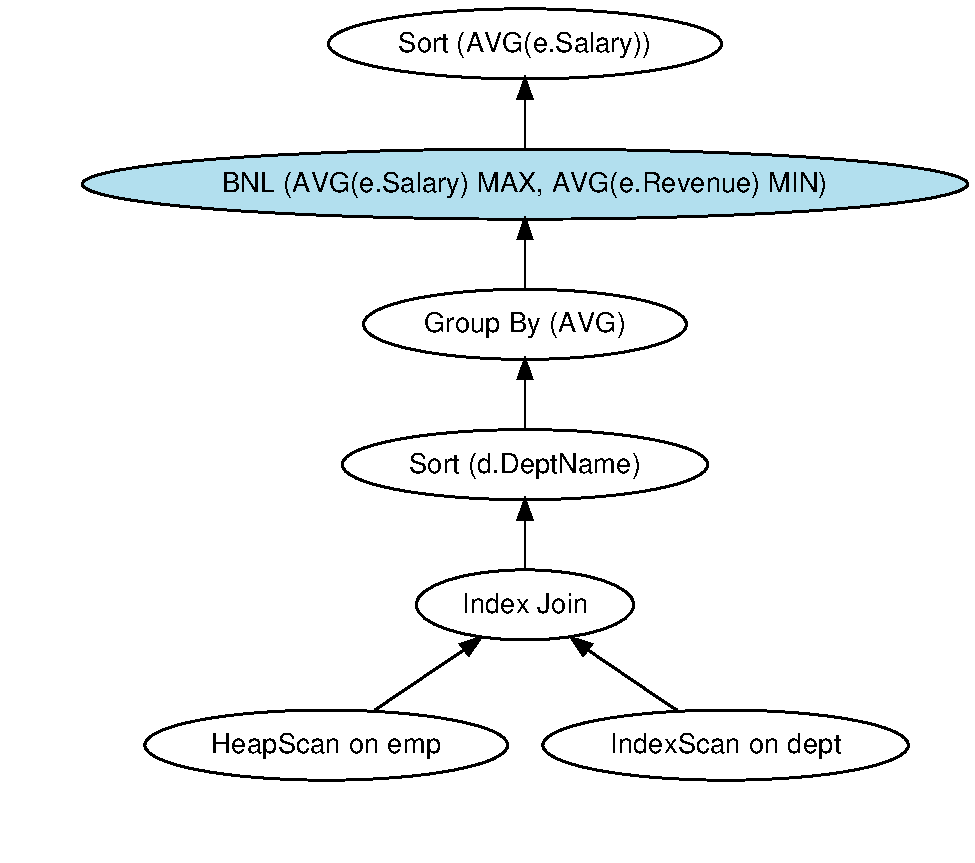
\includegraphics[scale=0.5]{plots-qp/qp-agg-bnl-sort}}\\
\subfloat[Query]{%
\parbox{100mm}{%
\texttt{%
SELECT d.DeptName, AVG(e.Salary), AVG(e.Revenue)\\
FROM emp e JOIN dept d on (e.Dno = d.DeptId)\\
GROUP BY d.DeptName\\
SKYLINE OF AVG(e.Salary) MAX, AVG(e.Revenue) MIN\\
ORDER BY AVG(e.Salary) DESC
}
}
}%
\caption{Example query plan for BNL}%
\label{fig:qp-agg-bnl-sort}%
\end{figure}

%

\begin{figure}[htbp]
\subfloat[BNL+EF]{%
\begin{minipage}[b]{\onecolumnwidth}%
\centering%
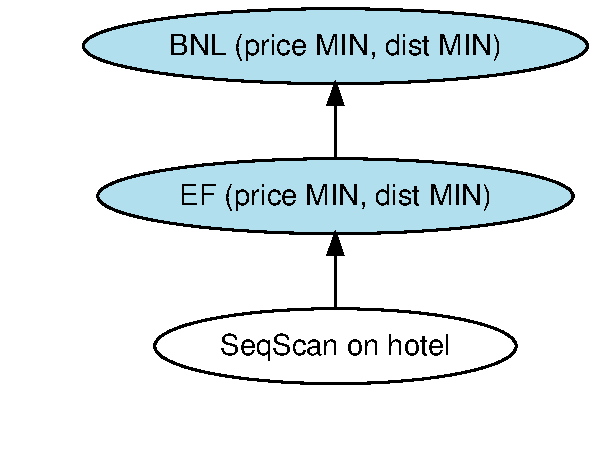
\includegraphics[scale=0.5]{plots-qp/qp-bnl-ef}%
\label{fig:qp-bnl-ef}%
\end{minipage}%
}%
\hspace{\columnsep}%
%
\subfloat[SFS+EF]{%
\begin{minipage}[b]{\onecolumnwidth}%
\centering%
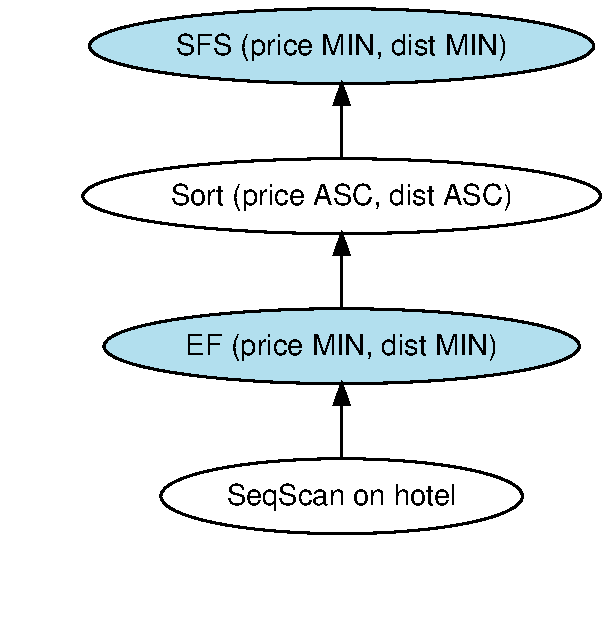
\includegraphics[scale=0.5]{plots-qp/qp-sfs-ef}%
\end{minipage}
\label{fig:qp-sfs-ef}%
}%
%
\\
%
\subfloat[SFS \emph{w/ index}]{%
\begin{minipage}[b]{\onecolumnwidth}%
\centering%
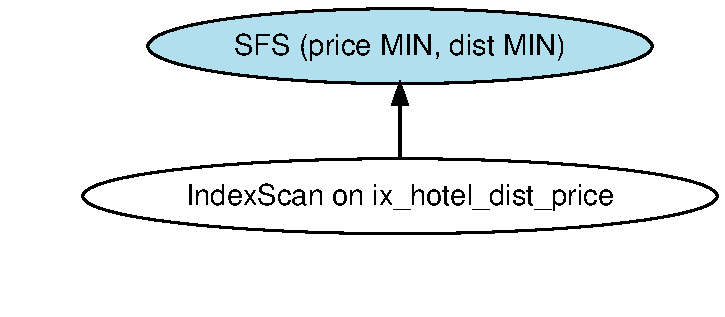
\includegraphics[scale=0.5]{plots-qp/qp-sfs-index}%
\label{fig:qp-sfs-index}%
\end{minipage}%
}%
\hspace{\columnsep}%
%
\subfloat[SFS+EF \emph{w/ index}]{%
\begin{minipage}[b]{\onecolumnwidth}%
\centering%
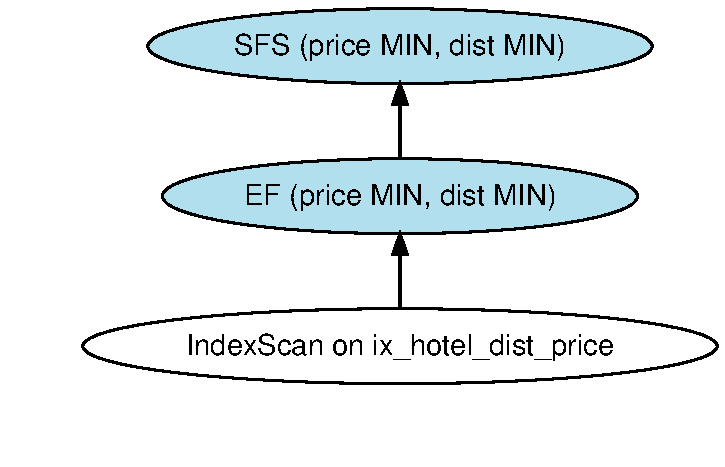
\includegraphics[scale=0.5]{plots-qp/qp-sfs-index-ef}%
\label{fig:qp-sfs-index-ef}%
\end{minipage}%
}%
\caption{Query plans for: 
\texttt{SELECT * FROM hotel SKYLINE OF price MIN, dist MIN;}}%
\end{figure}



\section{Pseudo Code}

\subsection{The stages of a query}

\subsection{The iterator model in the executor}

\subsection{Special case: one dimensional}
use is limited


\subsection{Special case: two dimensional with presort}
in case a suitable access path, no sort is needed,

brauchbar, da es unserer vermutung nach ein ein gut anzuwendender fall ist, aber d=2 macht skyline sinn.


\subsection{Tuple Window interface}

\subsection{BNL}

\subsection{SFS}

\subsection{Elimination Window EF and LESS}

\subsection{EF and BNL}

\section{Query base relation statistics}

PostgreSQL does not do a good job with statistics and subqueries.

\section{Cardinality and Cost Estimation}

cite \citep{Buchta1989}

\section{Usage of indizes}
skyline 1dim with index: in case of 1 dim skyline and the presence of
an usable index, the fact that the index scan could be cancled early
is not explored.

\section{\inlinesql{LIMIT} / \inlinesql{TOP $k$}}
how top k interacts with skyline, no special measures have to be taken
as the upper node will stop fetching tuples. only in cost estimation.


\section{Development}
\subsection{Debugging PostgreSQL}
During development it was very helpful to run the PostgreSQL backend
in \texttt{--single} mode. A single backend, enter the query directly,
edit \& continue in msvc.


\subsection{Regression Testing}
\todo{see \srcref{test/....}}{}
\todo{see more extensive see perl script}{}

\chapter{Results}
\label{chap:Results}


\section{Experimental Setup}
We ran our experiments on seven Dell OptiPlex 755, Intel Pentium
Dual-Core CPU E2160 (1.80GHz, 1MB L2 cache), with 1~GB RAM and Seagate
Barracuda 160~GB HDD (7200~rpm, SATA 3.0Gb/s, 8~MB cache) with a
single NTFS partition,
% average latency 4.16msec
running Microsoft Windows XP (SP2).
% 
Our implementation was based on PostgreSQL 8.3.0 and was compiled
using Microsoft Visual Studio 2005 (SP1) using the \texttt{RELEASE}
configuration with assertions disabled.
%
PostgreSQL was configured to use 200 MB of RAM for shared buffers,
with auto vacuuming disabled, and all other settings were left as
default.

If not otherwise mentioned, a tuple window size of 1024~KB (equal to
the PostgreSQL \texttt{work\_mem} setting), and an EF tuple window
size of 8~KB (equal to the PostgreSQL block size) were used.

The tables for the test runs have been generated using the extended
version \cite{Eder2007a} of the dataset generated presented in
\cite{Borzsonyi2001}, which allows to generate tables with
different initial seeds for the random generator. All experiments
were carried out on three different sets with varying initial seed, for each
distribution type (independent, correlated, and anti-correlated), and
with 100, 500, 1k, 5k, 10k, 50k, 100k tuples.

Each tuple consists of a unique 4 byte integer \emph{id} and 15
randomly generated 8 byte floats $d_1, \ldots, d_{15}$. With a 23 byte
tuple header and the alignment it sums up to a tuple length of 152 bytes. 
The memory chunk used by the PostgreSQL memory allocation function
(\texttt{palloc}) was 264 bytes long.
%The tuples are 152 bytes long, but the memory chunk used by PostgreSQL memory allocation function (palloc) is 264 bytes long.
%
%23 bytes tuple header, (0 bytes for null value bitmap) 
%
%data align at 8:
%4 (id) + 8 * 15 (d1-d15) = 124
%
%= 148 + alignment = 152
%
%MAXALIGN 
%MAXIMUM_ALIGNOF 8
%
%http://www.postgresql.org/docs/current/static/storage-page-layout.html

For the experiments using an index, a duplicate of the same set of
tables was used, including six indexes, where index $k$ is an index on
$d_1, \ldots, d_k$. This all sums up to 126 tables and an database of
approximately 1 GB.  
For most of our experiments we did not consider tables with more than
100k tuples, as the runtime for a 15 dimensional skyline query on 100k
tuples went up to 30 minutes.

% TODO hot cache, we ensure the table is in the shared buffer, before
% running the query, as each of the implemented methods has to read the
% entire table anyway

All experiments were carried out with a \emph{hot disk cache}, i.e. due to
appropriate queries all pages were in the shared buffers.


\subsection{Source Code}
Although we continously merging \texttt{CSV HEAD} of \fixme{PostgreSQL
source repository}{ref} into our main development branch, we decided
to base this paper on branch \texttt{REL8\_3\_STABLE}, in order to
have a more stable and reproducibly setting, i.e. all experiments in
this paper are based on version 8.3.0 of PostgreSQL with our patch for
the skyline operator applied.

\subsection{Lesson learned}
A lesson we have painfully learned during our experiments is to
minimize all possible influences on the runs to avoid skewed
results. This esspecially includes: screen savers, power saving or
standby options and any form of automatic software update suche as
Microsoft Windows Update or Google Pack software updater.

\subsection{Random Dataset Generator}

For our experiments we used a modified version \citep{Eder2007a} of
the popular dataset generator from \citep{Borzsonyi2001}.  Our
modified version can be used as command line utility or as a
PostgreSQL module. The PostgreSQL module provides a set returning
function and creates datasets on the fly.  The details are described
in the following sections.  But first of all we describe which type of
dataset are generated by the dataset generator.

\subsubsection{Independant, Correlated, and Anti-Correlated Datasets}
\label{sec:corr-anti-indep}

The main parameters one can vary for a generated dataset are
\emph{cardinality}, i.e. number of tuples, \emph{dimensionalty} and
the \emph{distribution type} and types are as of \citep{Borzsonyi2001}: 
\emph{independant}, \emph{correlated}, and \emph{anti-correlated}.

%Instead of giving a lenghty description of how the differnt
%distributions are generated, we present the essential parts of the
%source, as we believe this is the precisest way to describe it. Here
%are the some basic building blocks:

Before we give a detailed describtion of this distribution types, we
show some of the basic build blocks used for generating them, as we
believe the source code of the implementation is the precisest way to
describe it:

\begin{lstlisting}
static double
random_equal(double min, double max)
{
	double x = (double) rand() / RAND_MAX;
	return x * (max - min) + min;
}
\end{lstlisting}

As expected \lstinline{random_equal()} will return a random value $x
\in [\textnormal{min}, \textnormal{max}]$.

\begin{lstlisting}
static double
random_peak(double min, double max, int dim)
{
	int		d;
	double	sum = 0.0;

	for (d = 0; d < dim; d++)
		sum += random_equal(0, 1);
	sum /= dim;
	return sum * (max - min) + min;
}
\end{lstlisting}

The function \lstinline{random_peak()} returns a random value $x \in
[\textnormal{min}, \textnormal{max}]$ as sum of $\textnormal{dim}$
equally distributed random values.

\begin{lstlisting}
static double
random_normal(double med, double var)
{
	return random_peak(med - var, med + var, 12);
}
\end{lstlisting}

This function \lstinline{random_normal()} is our way to generate a
normally distributed value $x \in (\textnormal{med} -
\textnormal{var}, \textnormal{med} + \textnormal{var})$ with expected
value $E[x] = \textnormal{med}$.
%
This implementation is motivated through the central limit theorem and
based on the observation that a $12$-fold sum of $[0,1]$ uniformlly
distributed random value yields a sufficient good normally distributed
value. A prerequirement for this to work, is that the $12$ uniformlly
distributed values are intependent. While this can not be guaranteed
for \lstinline{random_equal()} we verified that data generated by
\lstinline{random_normal()} are sufficiently normally distributed with
the Shapiro-Wilk test.

Now we focus on the different distribution types and how they are
generated and we show some of their properties:

\begin{itemize}
\item \emph{indep}: 
for this type of dataset, all attribute values are generated
independently using a uniform distribution. Figure
\ref{fig:density-2d-i2d1e5} shows an density plot and statistics of
such an independent dataset with 100k tuples and $d = 2$. The skyline
tuples of this dataset are the lower left corners of the red line,
where the red line is the ``skyline''. The density of points within a
specific subregion is indicated by grayscale values, the darker the
more points are in the subregion. Above and to the right of the
grayscale density plot is the border distribution for each dimension,
in this plots the blue line indicates the density of a normal
distribution with the same mean and standard deviation as the border
distribution.

The implementation is as straight forward as expected:

\begin{lstlisting}
int		d;

for (d = 0; d < dim; d++)
	x[d] = random_equal(0, 1);
\end{lstlisting}

% TODO: place table and picture next to each other instead of below
\begin{figure}[htbp]
\centering
\sbox{\tempbox}{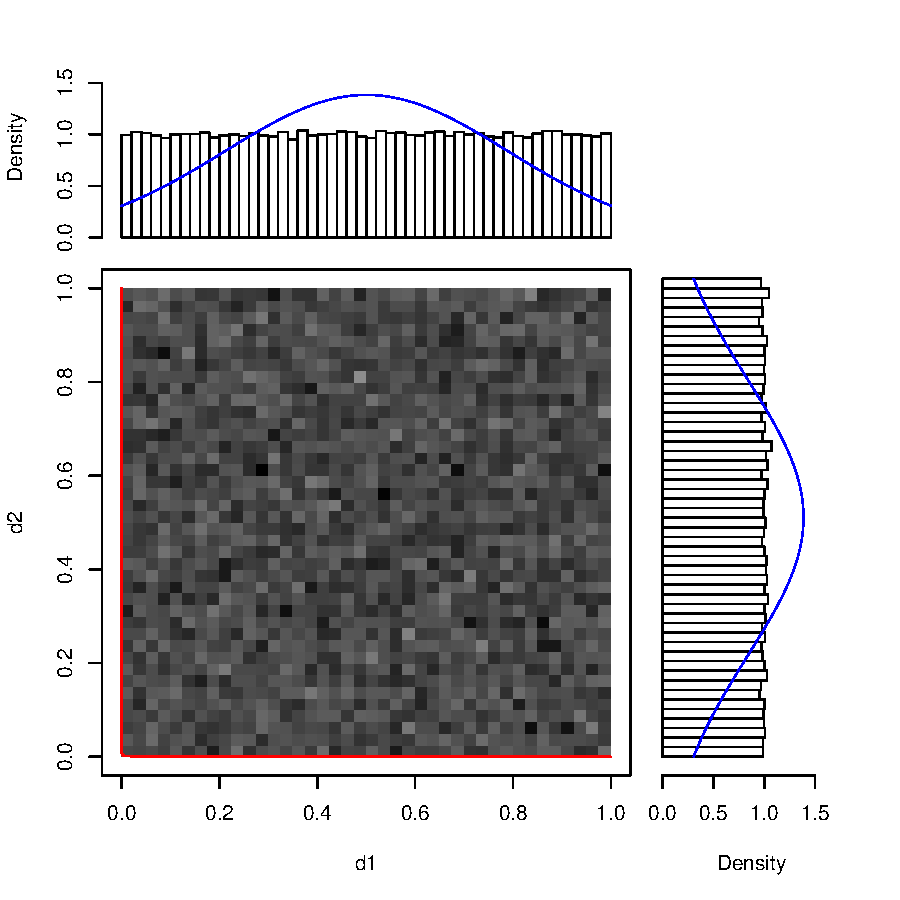
\includegraphics[width=100mm]{plots-density/density-2d-i2d1e5}}%
\subfloat[Density Plot]{\usebox{\tempbox}}%
\subfloat[Statistics]{%
\begin{minipage}[b]{38mm}%
\vbox to \ht\tempbox{%
\vfil
\begin{tabular}[b]{r|rr}%
	& d1 	& d2 \\
\hline
mean	& 0.500 & 0.500 \\
var	& 0.083 & 0.083 \\
\hline
cor	& d1	& d2 \\
\hline
d1	& 1.000 & 0.000 \\
d2	& 0.000 & 1.000 \\
\end{tabular}%
\vfil
}
\end{minipage}%
}%
\caption{Independent dataset (100k tuples)}%
\label{fig:density-2d-i2d1e5}%
\end{figure}

\item \emph{corr}: 
a correlated dataset represents an environment in which points which
are good in one dimension are also good in the other dimensions. 

%For instance, students which have a good publication record typically also
%do well in their preliminaries. 

A vextor $x$ with the dimension $dim$ is generated in the following way:

\begin{lstlisting}
do
{
	int		d;
	double	v = random_peak(0, 1, dim);
	double	l = v <= 0.5 ? v : 1.0 - v;
	
	for (d = 0; d < dim; d++)
		x[d] = v;

	for (d = 0; d < dim; d++)
	{
		double h = random_normal(0, l);
		x[d] += h;
		x[(d + 1) % dim] -= h;
	}
} while (!is_vector_ok(dim, x));
\end{lstlisting}

Due to the way it is computed an $x[d]$ could get out of the bound,
\lstinline{is_vector_ok()} verifies that all coordinates of $x$ are
within the interval $[0,1]$.

Figure \ref{fig:density-2d-c2d1e5} shows a correlated dataset with
100k tuples for $d = 2$.

\begin{figure}[htbp]
\centering
\sbox{\tempbox}{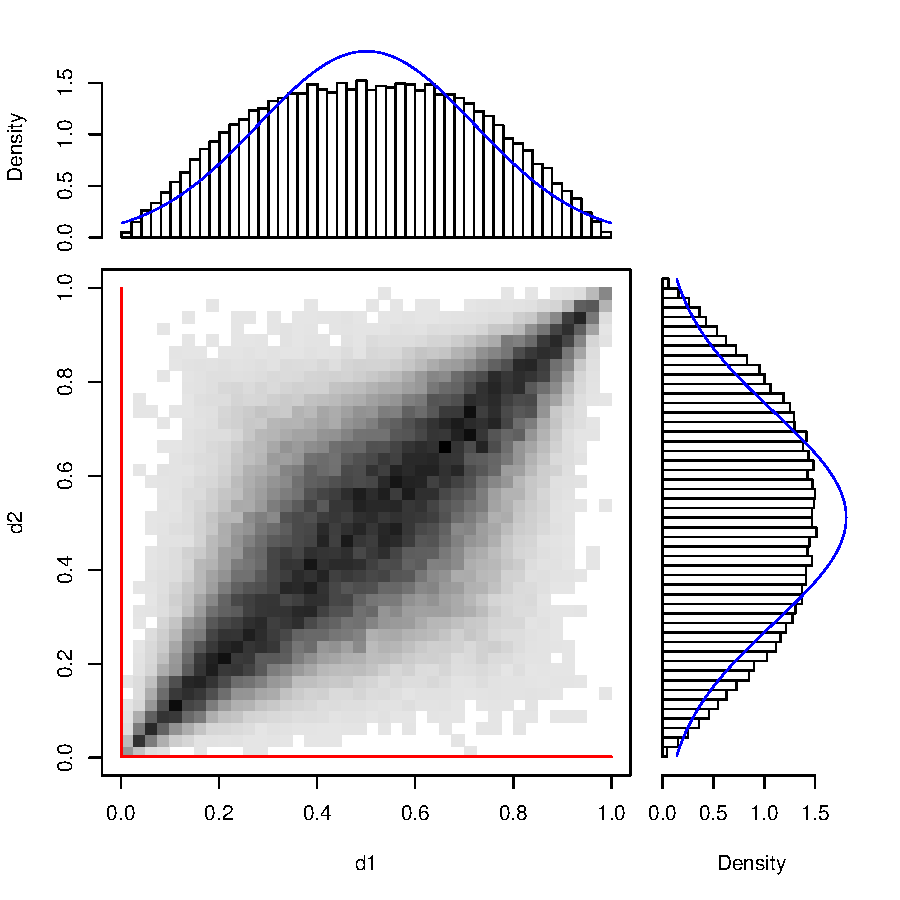
\includegraphics[width=100mm]{plots-density/density-2d-c2d1e5}}%
\subfloat[Density plot]{\usebox{\tempbox}}%
\subfloat[Statistics]{%
\begin{minipage}[b]{38mm}%
\vbox to \ht\tempbox{%
\vfil
\begin{tabular}[b]{r|rr}
	& d1 	& d2 \\
\hline
mean	& 0.500 & 0.500 \\
var	& 0.049 & 0.049 \\
\hline
cor	& d1	& d2 \\
\hline
d1	& 1.000 & 0.717 \\
d2	& 0.717 & 1.000 \\
\end{tabular}
\vfil
}
\end{minipage}
}
\caption{Correlated dataset (100k tuples)}%
\label{fig:density-2d-c2d1e5}%
\end{figure}


\item \emph{anti}:
an anti-correlated dataset represents an environment in which points
which are good in one dimension are bad in one or all of the other
dimensions. The standard example used in the skyline literature falls
into this category: hotels are either cheap and far away from the
beach or expensive and close to the beach.

\begin{lstlisting}
do
{
	int		d;
	double	v = random_normal(0.5, 0.25);
	double	l = v <= 0.5 ? v : 1.0 - v;
			
	for (d = 0; d < dim; d++)
		x[d] = v;
		
	for (d = 0; d < dim; d++)
	{
		double h = random_equal(-l, l);
		x[d] += h;
		x[(d + 1) % dim] -= h;
	}
} while (!is_vector_ok(dim, x));
\end{lstlisting}

Figure \ref{fig:density-2d-a2d1e5} shows an anti-correlated dataset
with 100k tuples for $d = 2$.
\end{itemize}

\begin{figure}[htbp]
\centering
\sbox{\tempbox}{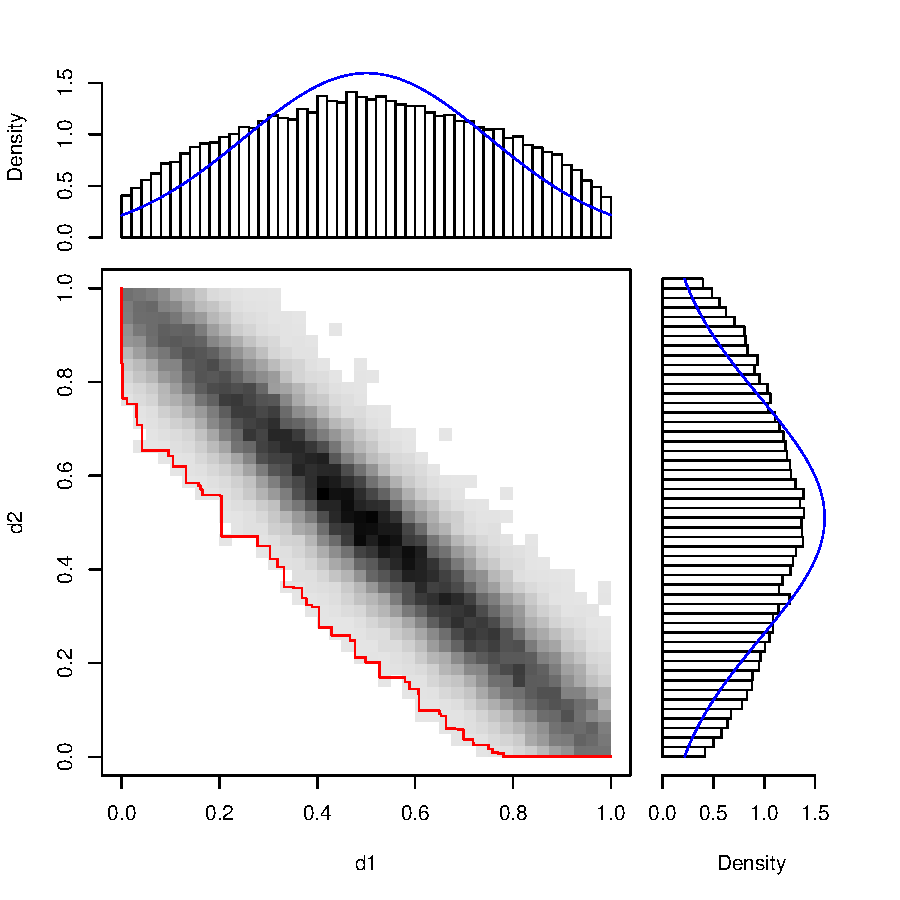
\includegraphics[width=100mm]{plots-density/density-2d-a2d1e5}}%
\subfloat[Density Plot]{\usebox{\tempbox}}%
\subfloat[Statistics]{%
\begin{minipage}[b]{38mm}%
\vbox to \ht\tempbox{%
\vfil
\begin{tabular}[b]{r|rr}
	& d1 	& d2 \\
\hline
mean	& 0.500 & 0.500 \\
var	& 0.063 & 0.063 \\
\hline
cor	& d1	& d2 \\
\hline
d1	& 1.000 & -0.944 \\
d2	& -0.9444 & 1.000 \\
\end{tabular}
\vfil
}
\end{minipage}
}
\caption{Anti-correlated dataset (100k tuples)}%
\label{fig:density-2d-a2d1e5}%
\end{figure}

For the very details of the random dataset generator, please have a
look at the implementation which is available from \citep{Eder2007a}.

\subsubsection{As command line utility}

The most benifitial use case for the command line version of the
random dataset generator is to pipe its output directly into the
database. The usage message explains how to use the command line
utility:

\begin{interactive}
\shprompt{randdataset -?}
Test Data Generator for Skyline Operator Evaluation
Usage: randdataset (-i|-c|-a) -d DIM -n COUNT [-s SEED] [-p] [-S] [-h|-?]

Options:
       -i       independent (dim >= 1)
       -c       correlated (dim >= 2)
       -a       anti-correlated (dim >= 2)

       -d DIM   dimensions >=1
       -n COUNT number of vectors
       -I       unique id for every vector
       -p PAD   add a padding field, PAD characters long

       -C       generate SQL COPY statement
       -R       generate SQL CREATE TABLE statement
       -T NAME  use NAME instead of default table name

       -s SEED  set random generator seed to SEED

       -S       output stats to stderr

       -h -?    display this help message and exit

Examples:
       randdataset -i -d 3 -n 10 -I -R
       randdataset -a -d 2 -n 100 -S
\end{interactive}

An invocation of \texttt{randdataset} suitable to pipe it directly
into \texttt{psql}, i.e. load it into database, could look like:

\begin{interactive}
\shprompt{randdataset -i -d 3 -n 10 -I -R}
DROP TABLE IF EXISTS "i3d10";
CREATE TABLE "i3d10" (id int, d1 float, d2 float, d3 float);
COPY "i3d10" (id, d1, d2, d3) FROM STDIN DELIMITERS ',' CSV QUOTE '''';
1,0.000000000000000e+00,6.900010321708401e-01,5.054183972559023e-01
2,5.914905399975788e-01,5.547849133400177e-01,3.784288188342139e-01
...\rcomment{7 rows omitted}
10,8.585111004572880e-01,9.898449857671955e-02,8.770675234855467e-01
\ttbackslash.
\end{interactive}

\subsubsection{PostgreSQL Random Dataset Generator Function}

To be able to generate test datasets on the fly, i.e. with out
explicitly creating tables and filling them up, we create a PostgreSQL
module which implements the functionality of \texttt{randdataset} as a
set returning function. To create, backup and restore a test database
with an appropriate set of test tables can be very time
consuming. Having such a function at had is useful in many situations,
all it takes is run PostgreSQLs \texttt{initdb} and install the set
returning function. We did so many times when merging PostgreSQL
8.3-devel branch into our branch, which often made it necessary to
re-\texttt{initdb}. Especially for regression tests and during
debugging this function was very handy. PostgreSQLs concept of
\postgresdocu{functions-srf.html}{set returning functions} allows to
issue queries as such:

\begin{interactive}
\sqlprompt{SELECT * FROM generate_series(2,4);}
 generate_series
-----------------
               2
               3
               4
(3 rows)
\end{interactive}

This concept of set returning functions is quite flexible and allows
also to return complex data types such as records. To test drive this
PostgreSQL 'contrib' module (see
\srcref(contrib/randdataset)), without installing it, even with
installing PostgreSQL visit our webinterface at
\url{http://skyline.dbai.tuwien.ac.at/}. To install it onto your
PostgreSQL installation follow the instructions
\srcref{contrib/randdataset/README.randdataset}. Once installed the
function can be used as follows:

\begin{interactive}
\sqlprompt{SELECT rds.id, rds.d1, rds.d2 FROM}\rcomment{columns are refered by name}
\sqlpromptcont{pg_rand_dataset('indep', 2, 10, 0) AS}\rcomment{2 dim independent dataset with 10 tuples}
\sqlpromptcont{rds(id int, d1 float, d2 float);}\rcomment{define names and types}
 id |         d1         |         d2
----+--------------------+--------------------
  1 |  0.170828036112165 |  0.749901980510867
  2 | 0.0963716553972902 |  0.870465227342427
...\rcomment{7 rows omitted}
 10 |  0.715538595204958 | 0.0830042460388524
(10 rows)

\sqlprompt{SELECT rds.* FROM}
\sqlpromptcont{pg_rand_dataset('corr', 3, 10, 0) AS}\rcomment{3 dim, correleted, 10 tuples}
\sqlpromptcont{rds(id int, d1 float, d2 float, d3 float);}
 id |        d1         |        d2         |        d3
----+-------------------+-------------------+-------------------
  1 | 0.482522432069401 | 0.327330244422693 | 0.207248995528228
  2 | 0.448836206689892 | 0.512027726159258 | 0.600054676092416
...\rcomment{7 rows omitted}
 10 | 0.319189108559988 | 0.407713612758059 |  0.30165467053249
(10 rows)

\sqlprompt{SELECT rds.* FROM}
\sqlpromptcont{pg_rand_dataset('anti', 3, 20, 1) AS}\rcomment{3 dim, anti-correlated, 20 tuples, seed 1}
\sqlpromptcont{rds(id int, d1 float, d2 float, d3 float);}
\comment{output ommit, as it is similar to above, except other distribution, more tuples, and another inital seed is used}
\end{interactive}

\noindent
The general signatur for \inlinesql{pg\_rand\_dataset} is:
\begin{interactive}
FUNCTION pg_rand_dataset(disttype text, dim int, rows int, seed int)
RETURNS setof record
\end{interactive}

\noindent
Where the arguments have following meaning:
\begin{itemize}
\item \texttt{disttype} specifies the distribution type (see section \ref{sec:corr-anti-indep}), allowed values are \texttt{'indep'}, \texttt{'corr'}, and \texttt{'anti'}

\item \texttt{dim} specifies the number of dimensions, allowed values are 1 upto 20 

\item \texttt{rows} specifies the number of tuples that should be returned, and 

\item \texttt{seed} is the seed for the random generator
\end{itemize}

We ensured that calling \inlinesql{pg\_rand\_dataset} with the same
arguments will always return the same result set. In the PostgreSQL
terminology this property of a function is called \texttt{IMMUTABLE}
(see PostgreSQL documentation on
\postgresdocu{xfunc-volatility.html}{Function Volatility Categories}).

To make the usage more comfortable we defined a set of wrapper
functions \texttt{rds$k$d} for the dimenions $k \in \{1, \ldots,
20\}$, they allowed us to issue the same queries as above in the
following why (see \srcref{contrib/randdataset/randdataset.sql.in}):

\begin{interactive}
\sqlprompt{SELECT rds.* FROM rds2d('indep', 10, 0) AS rds;}
\rcomment{output completely omitted, as it is the same as above}

\sqlprompt{SELECT rds.* FROM rds3d('corr', 10, 0) AS rds;}
\rcomment{same here}

\sqlprompt{SELECT rds.* FROM rds3d('anti', 20, 0) AS rds;}
\rcomment{same here}
\end{interactive}


\subsubsection{Buffer for Set returning function}

In the PostgreSQL execution engin a function scan node is responsible
for retrieving tuples from a set returning function. The current
implementation reads all the tuples from the set returning function
and stores them in a \texttt{tuplestore} before returning the first
tuple to the caller. A \texttt{tuplestore} maintains an in memory
buffer once it runs out of memory the remaining tuples are written to
a tempfile. The size of the in memory buffer is controlled through the
configuration variable \texttt{work\_mem}. The default value is
1024~KB. This configuration variable is also used to determine the amout
of RAM used for sort operations, for merge joins, hash joins and many more.
So RAM used for a single complex query can by multiple times the value of 
\texttt{work\_mem}.
In our setting we use the configuration variable \texttt{work\_mem}
for the sort operation in SFS and as the default tuple window size for
skyline algorithms that require a tuple window. In the following query
PostgreSQL call \texttt{generate\_series} a million times and will
discard all tuples except one due to the
\texttt{LIMIT 1}-clause.

\begin{interactive}
\sqlprompt{SELECT * FROM generate_series(1,1000000) LIMIT 1;}
 generate_series
-----------------
               1
(1 row)
\end{interactive}

This behavior is not desirable, at least we want that the tuples do
not get swapped out to disk as
\texttt{tuplestore}'s-\texttt{work\_mem} gets full, since for parts
of our experiments we were not willing to pay I/O penalty as we were
studing just the CPU bounded behavior of the skyline algorithms.

On the other hand we do not want to increase \texttt{work\_mem}, as
this would as mentioned above influence the sort operation and the size
of the tuple window for the skyline algorithms. Therefore we decided
to introduce a new configuration variable
\texttt{function\_scan\_work\_mem}, solely for the \texttt{tuplestore}
in the function scan node. The following utility query sets this
configuration variable to 100~MB;

\begin{interactive}
\sqlprompt{SET function_scan_work_mem  = 102400;}
\end{interactive}

\todo{}{link to the patch function\_scan\_work\_mem.diff}

\clearpage % \todo{remove clearpage}{}

\section{Comparisons and Analysis}
\label{sec:analysis}
We measure the time performance with respect to three parameters:
dimension, data cardinality, and data distribution.  We tested on the
following three data distributions: independent (i), correlated (c),
and anti-correlated (a).  For the other two factors "dimension" and
"cardinality", one has been fixed during each experiment.  Thus all
the plots are two dimensional.

\subsection{Time performance w.r.t. dimension}

\begin{figure}[htbp]
\centering%
\begin{minipage}{\onecolumnwidth}%
\subplotprofile[Independent dataset (100k tuples)]{bnl-wp-dim-i-100000}\\
\subplotprofile[Correlated dataset (100k tuples)]{bnl-wp-dim-c-100000}\\
\subplotprofile[Anti-correlated dataset (100k tuples)]{bnl-wp-dim-a-100000}%
\caption{Comparing runtime for different methods (100k tuples)}%
\label{fig:all-dim}%
\end{minipage}%
\hspace{\columnsep}%
\begin{minipage}{\onecolumnwidth}%
\subplotprofile[Independent dataset (100k tuples)]{all-dim-i-100000}\\
\subplotprofile[Correlated dataset (100k tuples)]{all-dim-c-100000}\\
\subplotprofile[Anti-correlated dataset (100k tuples)]{all-dim-a-100000}%
\caption{Absolute timing for different physical skyline operators (100k tuples)}%
\label{fig:all-dim-absolute}
\end{minipage}%
\end{figure}

For this set of experiments we fix the number of tuples of the input data.
Note that generally the absolute time measurements are not proportional 
throughout the dimensions, we thus deploy the relative values by setting one measurement as
the reference. 
In Figure~\ref{fig:all-dim-absolute}
we illustrate the absolute time measurements which are corresponding to
the relative values in Figure~\ref{fig:all-dim}. 
In the rest of the experiments, we only provide relative time measurements.

\todo{write about 2 dim case}{}

\subsubsection{Big datasets}
\label{sec:big-datasets}
Figure~\ref{fig:all-dim} shows the time performance of the skyline
algorithms vs. dimension with 100k tuples. It shows clearly that the
SFS+EF algorithm has the best time performance with all the data
distributions.  This conforms with the results in \cite{Godfrey2007},
where it was shown that LESS outperforms the SFS algorithm with 1M
tuples.

We also note that SFS performs extremely poor as the dimension is less
than six for independent and anti-correlated data, and even worse for
correlated data.  This can be justified that if the dimension is low,
the skyline selectivity factor\footnote{selectivity factor = skyline
tuples / input tuples. A low selectivity factor means high
selectivity.}  is low as well. Therefore, EF operation is effective,
i.e., a number of tuples could be removed at this stage. However, this
does not explain why SFS performs worse than BNL on datasets of low
dimensions. This can be clarified when considering the absolute time
measurement in Figure~\ref{fig:all-dim-absolute}.  It is shown that
the sorting routine of SFS has a nearly constant cost for all
dimensions. Therefore, for low dimensional datasets, the sorting cost
is dominant.

BNL+EF performs consistently better than BNL, due to the low skyline
selectivity factor for datasets with 100k tuples
(cf. Figure~\ref{fig:sf}).  As far as the window policy is concerned,
\emph{entropy} has consistently better performance for all the
algorithms.

\subsubsection{Small datasets}
\label{sec:small-datasets}

\begin{figure}[htbp]
\centering%
\begin{minipage}{\onecolumnwidth}%
\subplotprofile[Independent dataset]{presort-i}\\
\subplotprofile[Correlated dataset]{presort-c}\\
\subplotprofile[Anti-correlated dataset]{presort-a}%
\caption{Absolute timing for different physical skyline operators 
in the 2 dimensional case}%
\end{minipage}%
\hspace{\columnsep}%
\begin{minipage}{\onecolumnwidth}%
\subplotprofile[Independent dataset (1k tuples)]{bnl-wp-dim-i-1000}\\
\subplotprofile[Correlated dataset (1k tuples)]{bnl-wp-dim-c-1000}\\
\subplotprofile[Anti-correlated dataset (1k tuples)]{bnl-wp-dim-a-1000}%
\caption{Comparing runtime for different methods (1k tuples)}
\label{fig:all-dim-onek}
\end{minipage}%
\end{figure}

Figure~\ref{fig:all-dim-onek}
depicts the time-dimensionality performance regarding to datasets with 1k number of tuples.
One interesting observation is that the performance of SFS 
is surprisingly better than others, except for the extremely low dimension values
(three for independent, anti-correlated, and six for correlated distributions).
As illustrated by Figure~\ref{fig:sf}, 
there exists a causal relation with the skyline selectivity factors.
It shows clearly that as the data cardinality decreases,
the skyline selectivity factor increases. Therefore, in general, the EF operator is less effective 
with lower data cardinalities. To be more accurate, if the skyline selectivity factor
is higher than 0.1, the benefit gained from EF is marginal. 
This is confirmed by the results shown in Figure~\ref{fig:all-dim} as well.

The result is somehow contradictory to the claim that SFS+EF should 
perform consistently better than SFS, because at the EF stage there should be always 
some tuples eliminated. However, one should not ignore the cost of the EF operation,
where comparisons are executed. Moreover, if the \emph{entropy} window 
policy is applied, the time consumption is even higher. Hence, there exist
data settings where EF does not pay off anymore.

\subsection{Time performance w.r.t. cardinality}

To better understand the time performance of the skyline algorithm
with respect to the data cardinality, 
we conducted experiments for each dimension $k \in \{2, \ldots, 15\}$
with the number of tuples ranging from 100 to 100k. 
For each data distribution we have chosen four to five representative
dimension values.
Figure~\ref{fig:inde}, \ref{fig:corre}, and \ref{fig:anti}
illustrate the test results for independent, correlated,
and anti-correlated datasets, respectively.

Surprisingly, the \emph{rule of the selectivity factor} 
is proven to be true in all the datasets. 
That is, 
if the selectivity factor is higher than 0.1, the elimination filter
does not have any advantage. 

\subsubsection{Independent and anti-correlated datasets}
Let us first consider the independent datasets (Figure~\ref{fig:inde}).
As the dimension is higher than four, SFS is superior for all datasets,
except for data cardinality of 50k and 100k, where SFS+EF outperforms SFS.
If we examine again the selectivity factor for independent datasets in Figure~\ref{fig:sf},
these datasets are in the category where the selectivity factor 
is higher than 0.1. This result confirms our observation in Section~\ref{sec:small-datasets}.
Note that the same observation holds for BNL+EF vs. BNL as well.

With dimension three there is an exception, where BNL performs best.
This can be justified as follows: 
the sorting cost remains constant w.r.t. dimensions,
thus it becomes dominant with low dimension (such as three). 

The performance of anti-correlated datasets in Figure~\ref{fig:anti} 
behaves similarly to that of independent datasets, 
thus the above analysis can be applied as well.

\subsubsection{Correlated datasets}
For correlated datasets in Figure~\ref{fig:corre}, SFS+EF is superior
with a few exceptions. This again, can be perfectly explained by
the selectivity factors for correlated datasets (cf. Figure~\ref{fig:sf-c}).
Except for the data cardinality of 100 and 500, all
the selectivity factors are remarkably low (most of them are less than 0.1),
thus the EF operation pays off.

\begin{figure}[htbp]
\centering%
\subplotprofile[3 dim (independent)]{bnl-wp-rows-i-03}%
\hspace{\columnsep}%
\subplotprofile[4 dim (independent)]{bnl-wp-rows-i-04}\\
\subplotprofile[6 dim (independent)]{bnl-wp-rows-i-06}%
\hspace{\columnsep}%
\subplotprofile[9 dim (independent)]{bnl-wp-rows-i-09}\\
\subplotprofile[15 dim (independent)]{bnl-wp-rows-i-15}%
\caption{Comparing runtime for independent datasets}%
\label{fig:inde}%
\end{figure}

\begin{figure}[htbp]
\centering%
\subplotprofile[3 dim (correlated)]{bnl-wp-rows-c-03}%
\hspace{\columnsep}%
\subplotprofile[5 dim (correlated)]{bnl-wp-rows-c-05}\\
\subplotprofile[8 dim (correlated)]{bnl-wp-rows-c-08}%
\hspace{\columnsep}%
\subplotprofile[15 dim (correlated)]{bnl-wp-rows-c-15}%
\caption{Comparing runtime for correlated datasets}%
\label{fig:corre}%
\end{figure}


\begin{figure}[htbp]
\centering%
\subplotprofile[3 dim (anti-correlated)]{bnl-wp-rows-a-03}%
\hspace{\columnsep}%
\subplotprofile[4 dim (anti-correlated)]{bnl-wp-rows-a-04}\\
\subplotprofile[7 dim (anti-correlated)]{bnl-wp-rows-a-07}%
\hspace{\columnsep}%
\subplotprofile[15 dim (anti-correlated)]{bnl-wp-rows-a-15}%
\caption{Comparing runtime for anti-correlated datasets}%
\label{fig:anti}%
\end{figure}


\begin{figure}[htbp]
\centering%
\begin{minipage}{\onecolumnwidth}%
\subplotlabeledprofile{Independent dataset (100k tuples)}{sfs-index-i-100000}{fig:sfs-index-i}\\
\subplotlabeledprofile{Correlated dataset (100k tuples)}{sfs-index-c-100000}{fig:sfs-index-c}\\
\subplotlabeledprofile{Anti-correlated dataset (100k tuples)}{sfs-index-a-100000}{fig:sfs-index-a}%
\caption{Relative timing for SFS/SFS+EF when using index access paths (100k tuples)}%
\label{fig:sfs-index}%
\end{minipage}%
%\hspace{\columnsep}%
%\begin{minipage}{\onecolumnwidth}%
%\subplotlabeledprofile{independent dataset}{selectivity-dim-i}{fig:sf-i}\\
%\subplotlabeledprofile{correlated dataset}{selectivity-dim-c}{fig:sf-c}\\
%\subplotlabeledprofile{anti-correlated dataset}{selectivity-dim-a}{fig:sf-a}%
%\caption{Skyline operator selectivity factor on our test datasets}%
%\label{fig:sf}%
%\end{minipage}
\end{figure}


\begin{figure}[htbp]
\centering%
\begin{minipage}{\onecolumnwidth}%
\subplotlabeledprofile{Independent dataset}{selectivity-dim-i}{fig:sf-i}\\
\subplotlabeledprofile{Correlated dataset}{selectivity-dim-c}{fig:sf-c}\\
\subplotlabeledprofile{Anti-correlated dataset}{selectivity-dim-a}{fig:sf-a}%
\end{minipage}%
\hspace{\columnsep}%
\begin{minipage}{\onecolumnwidth}%
\subplotlabeledprofile{Independent dataset}{selectivity-rows-i}{fig:sf-rows-i}\\
\subplotlabeledprofile{Correlated dataset}{selectivity-rows-c}{fig:sf-rows-c}\\
\subplotlabeledprofile{Anti-correlated dataset}{selectivity-rows-a}{fig:sf-rows-a}%
\end{minipage}
\caption{Skyline operator selectivity factor on our test datasets}%
\label{fig:sf}%
\end{figure}


\begin{figure}[htbp]
\centering
\subplotlabeledprofile{1k tuples}{ef-eff-dim-1000-efws8}{fig:ef-eff-1k}\\
\subplotlabeledprofile{10k tuples}{ef-eff-dim-10000-efws8}{fig:ef-eff-10k}\\
\subplotlabeledprofile{100k tuples}{ef-eff-dim-100000-efws8}{fig:ef-eff-100k}%
\caption{Effectiveness of elimination filter (EF) for varying dimensions}%
\label{fig:ef-eff}%
\end{figure}

\subsection{SFS using indexes}
The idea is to leverage the index structure for SFS in order to avoid an explicit sort.
For SFS+EF w/ index this is illustrated in Figure~\ref{fig:qp-sfs-index-ef}.
It is up to the query optimizer to decide by means of cost estimation 
whether to use an index or not.
We analyzed the usage of indexes for SFS in detail for 100k tuples 
(see Figure~\ref{fig:sfs-index}).

It turns out that SFS w/ index consistently outperforms SFS, 
independent from the window policy used, with a single exception (cf. 
Figure~\ref{fig:sfs-index-a} when dim=6). 
This is clearly an argument for using an index.

However, SFS+EF w/ index performs worse than SFS w/ index. 
This is somehow counterintuitive, because for 100k tuples 
SFS+EF performs better than SFS, as we have discussed
in Section~\ref{sec:big-datasets} (cf. Figure~\ref{fig:all-dim}).
We argue that, the effectiveness of EF deteriorates
in the presence of the index structure.
The data is physically ordered according to one of the indexed attributes,
which is not guaranteed to be beneficial for the elimination filtering.
Therefore, one should be careful with applying EF in the presence of index,
even on the datasets with low selectivity factors.
%
The only significant exception is for correlated data, window policy append, and dim 
$\le 3$ (cf. Figure~\ref{fig:sfs-index-c}).
We argue this is due to the general low selectivity factor and high EF effectiveness in 
this case (cf. Figure~\ref{fig:sf-c} and \ref{fig:ef-eff-100k}).

In all aspects, SFS w/ index and SFS+EF w/ index are outperformed
by SFS+EF using window policy entropy or prepend. This can
be explained with the same argument as above, EF eliminates
so many tuples prior to sorting that this becomes cheaper than
using an index.

%\pagebreak[4]
\subsection{Window policy}
All experimental results show that the \emph{entropy} is
the most efficient and effective window policy.
One might notice that on correlated datasets, the \emph{prepend}
window policy performs the worst in the SFS algorithm. 
The explanation is obvious: if the correlated data is sorted,
the most effective skyline tuples (that is, the tuples dominate 
most of the other tuples) tend to enter the widow earlier. 
However with the prepend policy, these tuples are successively pushed
to the end of the window, which results in high time costs
for checking whether a new tuple is dominated by
the tuples in the window.
Figure \ref{fig:ef-eff} shows that \emph{entropy} is
the most effective EF window policy. 



\subsection{Parameter Space}
\todo{see \citep{Gray1993}}{}

There is a large number of parameters that can be varied:

\begin{itemize}
\item \emph{size of dataset} (100?, 1000?, 10000, 100000, 1000000)
\item \emph{number of dimensions} (1-15, or even 10 is enough)
\item \emph{data distribution} (indep, corr, anti)
\item \emph{data source} (disk, set returning function)

in case the data are stored on disk
\begin{itemize}
\item \emph{sequencial scan vs. index scan} SFS can benefit from index scan (ommit sort phase), BNL and SFS could benefit from a index scan if DIFF groups are used.
\item \emph{sequence of tuples in tuple stream} (random, high entropy first/last) for BNL and EF if a very good tuple is very early in the tuple stream it will eliminate a lot of tuples in a very early stage
\end{itemize}
\item \emph{methods}

\begin{itemize}
\item as SQL statement
\item special case 1 dim distinct
\item special case 1 dim 
\item special case 2 dim (needs sort presort or access path)
\item BNL
\item SFS
\item EF+SFS=LESS
\item EF+BNL
\end{itemize}

\item window size
\item window policy (prepend, append, entropy)
\item entropy needs stats for scaling to (0,1)

\end{itemize}

Todo's

\begin{itemize}
\item use 90\% percentile (\citep{Gray1993}[page 315]) vs, average / variance (box-plots?)
\item describe software (operating system: Windows XP + SP 2, Microsoft Visual Studio 2005 + SP1, based on PostgreSQL 8.3.0) and hardware (CPU, RAM, Disk config, File System) used for benchmarking

\item describe the configuration of PostgreSQL (flags used for \texttt{configure --enable-asserts --enable-checks, ...}, it is recommended to turn asserts and co. off for benchmarking
\end{itemize}


\subsection{window size}
assumtions on windowsize:

the assumtion that at no time more than output\_tuples will be in the
window can not be hold.

larger window and and less passes do not always mean better runtime

infact there is a break even point

\subsection{Special case 1 dim skylines}


\subsection{Special case 2 dim skylines}

%%
%% Summary
%%

\chapter{Summary}
%\addcontentsline{toc}{chapter}{Summary}

\section{Futher work}

\subsection{Speedups for low cardinalty domains}
%
use special algorithms if we deal with domains with small
cardinalites, \citep{Preisinger2006, Preisinger2007, Morse2007}

\subsection{Speedups for \inlinesql{SKYLINE OF DIFF}}
%
Use a seperate tuple window for each \inlinesql{SKYLINE OF DIFF}
group, so only the tuples with the same values on the
\inlinesql{SKYLINE OF DIFF} attributes have to be compared to each
other. This reduction of comparision would yield an overall speedup.
In order to avoid an unbounded number of tuple windows instead of
having a tuple window for each \inlinesql{SKYLINE OF DIFF} group
hashing could be engaded, i.e. allocate a fixed number of tuple
windows and hash each \inlinesql{SKYLINE OF DIFF} group into one tuple
window.

\subsection{Extensions}

\subsubsection{Sampling}

In the absence of statistics for the relation in questions, sampling
could be engadged. \todo{cite}{Chaurduri2006}

\subsubsection{$K$-skyband}
implement $K$-skyband (maintaine dominance count in tuple window) do
so for BNL and SFS.

\subsubsection{$k$-dominance skyline}
\todo{is this easy possible?}{}






